\documentclass[12pt,a4paper]{report}

\usepackage[spanish]{babel}
\usepackage[utf8]{inputenc}
\usepackage{dad}
\usepackage{pdfpages}

\title{Desarrollo de Aplicaciones Distribuidas: \\ Registrador de juegos}
\author{Rafael Gálvez-Cañero, Andreas Gerstmayr}
\date{Iteración 5 - 28 de Abril de 2015} % delete this line to display the current date



%%% BEGIN DOCUMENT
\begin{document}
\maketitle
\tableofcontents
\listoffigures
\listoftables

\pagenumbering{arabic}

% Esto representa la primera iteración (capítulo), información general
\chapter{Datos generales}

\section{Miembros del grupo}

\begin{table}[htdp]
\begin{center}
\begin{tabular}{|l|l|l|c|}
\hline
\textbf{Apellidos}&\textbf{Nombre}&\textbf{Correo-e}&\textbf{Grupo}\\
\hline
Gálvez-Cañero&Rafael&\href{mailto:galvesband@gmail.com}{galvesband@gmail.com}&18\\
Gerstmayr&Andreas&\href{mailto:andreas.gerstmayr@gmail.com}{andreas.gerstmayr@gmail.com}&18\\
\hline
\end{tabular}
\end{center}
\caption{Miembros del grupo}
\label{tab:miembros}
\end{table}%


\section{Descripción del sistema}

\begin{itemize}
\item \textbf{Tipo de sistema distribuido}: Sistema de información.
\item \textbf{Nombre del proyecto}: Plataforma de juegos, Game Registry.
\item \textbf{Breve descripción}: Sub-sistema para registrar sesiones de juego e información asociada.
\end{itemize}

\subsection{Funcionalidad observable}

\begin{itemize}
\item Registrar el inicio y el término de todas las sesiones de juego.
\item Visualizar el historial de juegos.
\end{itemize}

\subsection{Servicios ofrecidos}
\begin{itemize}
\item Servicio de Registro: Capacidad de aceptar la información de una sesión de juego (juego ID, jugador ID y fecha de inicio y término).
\item Servicio de Historial: Ofrece métodos para consultar el historial de sesiones.
\end{itemize}

\subsection{Servicios demandados}
\begin{itemize}
\item Servicio de Juego: avisar de término de una sesión de juego
\item Servicio de Juego: recibir el título de un juego
\item Servicio de Perfil: rebibir el nombre de un jugador
\end{itemize}

\section{Direcciones de descarga y planificación}

\begin{table}[htdp]
\begin{center}
\begin{tabular}{|c|c|}
\hline
\textbf{Código fuente}&\url{https://repositorio.informatica.us.es/svn/lq3vqrtzfnh2nx9yhpk}\\
\hline
\multicolumn{2}{|c|}{\textbf{Planificación temporal}}\\
\hline
Iteración 1&24/02/2015\\
Iteración 2&03/03/2015\\
Iteración 3&26/03/2015\\
Iteración 4&7/04/2015\\
Iteración 5&28/04/2015\\
Iteración 6&12/05/2015\\
Iteración 7&26/05/2015\\
Entrega Final&02/06/2015\\
\hline
\end{tabular}
\end{center}
\caption{Datos generales del trabajo en grupo}
\label{tab:datosgenerales}
\end{table}%

\section{Seguimiento}

\begin{table}[htdp]
\begin{center}
\begin{tabular}{|c|c|c|c|c|c|c|c|c|c|c|}
\cline{2-9}
\multicolumn{1}{c}{}&\multicolumn{8}{|c|}{\textbf{Iteración}}&\multicolumn{2}{c}{}\\
\hline
\textbf{Estudiante}&1&2&3&4&5&6&7&Final&Total&Pond.\\
\hline
Rafael Gálvez-Cañero&5&5&5&5&-&-&-&-&\textbf{20}&1\\
Andreas Gerstmayr   &5&5&5&5&-&-&-&-&\textbf{20}&1\\
\hline
Total               &10&10&10&10&0&0&0&\multicolumn{2}{c}{}\\
\cline{1-8}
\end{tabular}
\end{center}
\caption{Tabla de seguimiento}
\label{tab:seguimiento}
\end{table}%


% Segunda iteración (capítulo), diagramas UML de clases y despliegue
\chapter{Modelado}

\section{Análisis del sistema}
 \begin{center}
  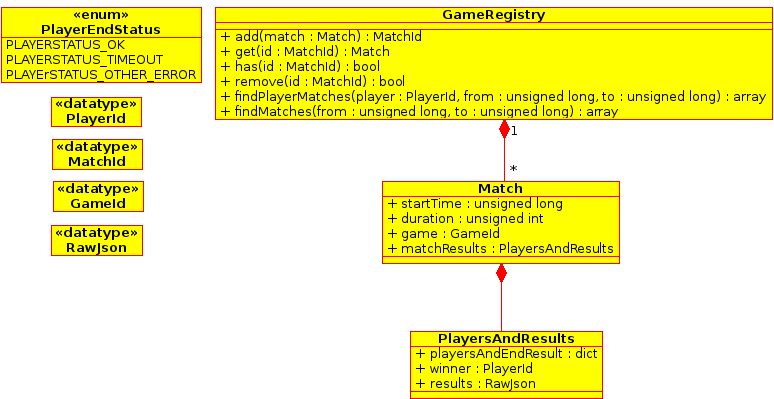
\includegraphics[scale=0.6]{./class_diagram.png}
  % class_diagram.png: 0x0 pixel, 300dpi, 0.00x0.00 cm, bb=
 \end{center}


\section{Arquitectura del sistema}
\begin{figure}[center]
 \missingfigure{TODO}
 \caption{Modelo de despliegue del sistema}
 \label{fig:arquitectura}
\end{figure}


% Tercera iteración (gradle, dockerización)
\chapter{Iteración 3}
\section{Objetivos de iteración}
\begin{itemize}
  \item Integración de Gradle 
  \item Servidor dockerizado
  \item Estructura inicial del Cliente vertx.
\end{itemize}

\section{Gradle}
\emph{Gradle} es un gestor de construcción especialmente indicado para proyectos
Java y con soporte para \emph{Groovy}, \emph{Vertx} y \emph{Maven}.

Ha sido integrado mediante el wrapper \texttt{gradlew} que permite utilizar Gradle sin
instalarlo de forma global en el sistema de desarrollo. La primera vez que se
lanza descargará todas las bibliotecas necesarias.

En el archivo \textbf{Readme.md} hay información básica sobre como construir el
proyecto. Algunos comandos útiles:

\begin{itemize}
 \item Para \textbf{construir} el proyecto: \\
       \texttt{\$ ./gradlew clean modZip}
 \item Para \textbf{lanzar} el servidor en la máquina local: \\
       \texttt{\$ ./gradlew runMod -i}
 \item Para lanzar los \textbf{tests}: \\
       \texttt{\$ ./gradlew clean test}
 \item Para preparar el proyecto para un \textbf{entorno de desarrollo}:
    \begin{itemize}
      \item Eclipse: \texttt{\$ ./gradlew eclipse}
      \item IDEA: \texttt{\$ ./gradlew idea}
    \end{itemize}
\end{itemize}

\section{Dockerización}
\emph{Docker} es una tecnología que permite utilizar contenedores sobre \emph{Linux} para
ejecutar procesos de forma aislada y con un runtime reproducible.

Nuestro proyecto proporciona un archivo \textbf{Dockerfile} con las instrucciones necesarias
para construir el contenedor de la aplicación. Además, el archivo \textbf{Readme.md} contiene
información sobre el procedimiento para lanzar el proyecto en \emph{Docker}. 

El procedimiento para lanzar el servidor con \emph{Docker} ahora mismo es el siguiente:

\begin{itemize}
 \item Limpiar y contruir el proyecto: \\
       \texttt{\$ ./gradlew clean modZip}
 \item Construir el contenedor con el servidor: \\
       \texttt{\$ docker build -t distributedsystems/gameregistry .} \\
       (notar el punto final del comando que indica a \emph{Docker} dónde buscar el archivo
       \emph{Dockerfile} con las instrucciones de construcción). La construcción incluye el 
       resultado de compilación del proyecto por lo que cada vez que este cambie el contenedor
       debe ser reconstruido.
 \item Lanzar el contenedor del servidor: \\
       \texttt{\$ docker run distributedsystems/gameregistry}
\end{itemize}


% Cuarta iteración (mongo, reestructuración de servidor en Servicio / Controlador / Dominio)
%!TEX root =  MemoriaGrupo00.tex
% --------------------------------------------
% Iteraci�n 4
% --------------------------------------------
\chapter{Iteraci�n 4}

\section{Planificaci�n}
\section{Dise�o}
\subsection{Diagrama de clases UML}

\begin{figure}[htbp]
\begin{center}
\missingfigure{Aqu� el modelo de dise�o en formato vectorial preferentemente (pdf)}
% Incluir la figura quitando el comentario a la fila de abajo.
% \includegraphics[width=\textwidth]{myfile.pdf}
\caption{Diagrama UML de dise�o para la iteraci�n 4}
\label{fig:diseno03}
\end{center}
\end{figure}

\subsection{Documentos de asignaci�n de responsabilidades}

\subsection{Memorandos t�cnicos}

\section{Informaci�n adicional}


% Quinta iteración (API inicial, primeros test, despliegue en azure, investigacion integración contínua.
\chapter{Iteración 5}
\section{Objetivos de iteración}
\begin{itemize}
  \item Definición de API en Swagger
  \item Implementación inicial de API REST
  \item Primeros tests
  \item Despliegue en plataforma Azure
  \item Investigar integración contínua
\end{itemize}


\section{Definición de API en Swagger}
TODO URL a Swagger y a wiki de projetsii, etc


\section{Implementación inicial de API REST}
TODO Contar algo de SessionController, SessionsController y la API


\section{Primeros tests}
TODO  Contar qué tests hay, más o menos.


\section{Despliegue en plataforma Azure}
Tras evaluar las opciones de despliegue de \emph{Docker} en \emph{Azure} hemos
optado por construir una máquina virtual donde administraremos manualmente una
instancia de \emph{Docker} en vez de utilizar la extensión de máquina virtual
que implementa \emph{Azure} para \emph{Docker}. Utilizar esta última habría implicado
una complejidad añadida por la parafernalia necesaria para mantener certificados de
seguridad para poder comunicarnos con la instancia de  \emph{Docker}.

En lugar de la extensión de máquina virtual de \emph{Azure} administraremos la 
máquina virtual manualmente.


\subsection{Test vm}
Para esta iteración hemos creado una máquina virtual cuyo propósito es familiarizarnos
con el entorno \emph{Azure}. Para ello los requisitos de esta máquina serían:

\begin{itemize}
 \item Ser capaz de ejecutar el servidor \emph{GameRegistry} y \emph{MongoDB} como
       contenedores de \emph{Docker}.
 \item Ser capaz de construir el contenedor de \emph{GameRegistry} a partir del 
       repositorio SVN del proyecto.
\end{itemize}

Para ello se ha basado la máquina virtual en una imagen de \emph{Ubuntu 15.04}, que contiene
una versión reciente y razonablemente testada de \emph{Docker}. Además hemos añadido
el cliente de \emph{Subversion} y el \emph{OpenJDK-8}.


\subsection{VM de producción}
Aún no creada. Sus requisitos son similares pero no iguales a la máquina test. El propósito
de esta máquina virtual será el de ejecutar el servidor, evitando la instalación
de cualquier pieza de software no necesaria para esa tarea, lo cual en este caso implica
no instalar ningún \emph{JDK} ni \emph{Subversion}.

Esto requiere algún método para hacer llegar el contenedor con el servidor GameRegistry a
la máquina que no implique a \emph{Subversion} ni el uso de \emph{Java} para compilar
el código fuente. Lo resolveremos en la próxima iteración.

\begin{figure}[h]
 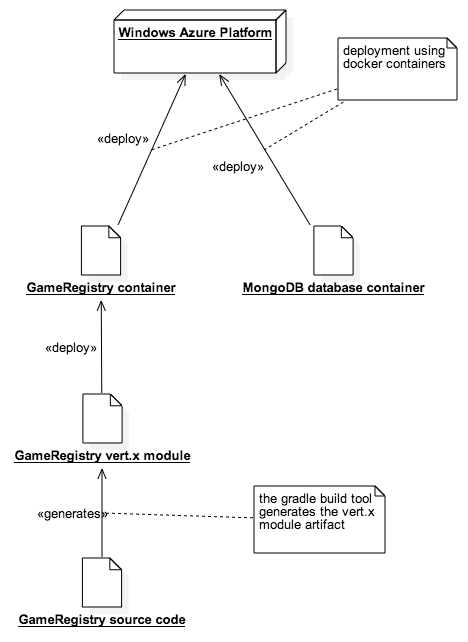
\includegraphics[scale=0.6]{diagrams/docker_deployment_diagram.png}
 \caption{Diagrama de despliegue (iteración 5)}
 \label{fig:despliegue}
\end{figure} 


\section{Investigar integración contínua}
Algún método de integración contínua sería interesante para el proyecto de forma que los tests 
sean ejecutados en cada revisión del proyecto. Hay sitios web que ofrecen una instancia gratuita de
integración contínua que podrían ser utilizados, como por ejemplo:

\begin{itemize}
\item CircleCI (\texttt{https://circleci.com/})
\item CodeShip (\texttt{https://codeship.com/})
\end{itemize}

Estamos aún estudiando la viabilidad y los requisitos impuestos.
 
\chapter{Iteracion 6}
\section{Objetivos de iteración}
\begin{itemize}
 \item Integración de documentación de Swagger en la memoria y el proyecto.
 \item Reestructuración de los contenedores para hacer más sencillo el despliegue en Azure
 \item Máquina virtual de producción, procedimiento de despliegue determinado.
 \item Testing.
\end{itemize}

\chapter{Iteracion 7}
\section{Objetivos de iteración}
Subir a repositorio Maven.

\chapter{Documentación de API GameRegister}
\includepdf[pages={-}]{../gameregistry/build/docs/apidoc/pdf/apidoc.pdf}

\end{document}
